\documentclass[twocolumn]{IEEEtran}
\usepackage{amsmath}
\usepackage{graphics}
\usepackage{graphicx}
\usepackage[english]{babel}



%opening
\begin{document}
\title{DESCAD: an OOP based tool for Automated Electronic Design}
\author{Roberto Casta\~neda-Sheissa, Arturo Sarmiento-Reyes, Luis Hern\'andez-Mart\'inez, H\'ector V\'azquez-Leal}

\maketitle
\thispagestyle{empty}
\pagestyle{empty}
\begin{abstract}
Computer aided design (CAD) tools allows a user/developer to execute complex tasks, resolve difficult calculations, or optimize processes with minimum effort. CAD tools are present in many fields like chemistry, physics, mathematics, astrophysics, engineering, and electronics. For electronics, most of the available CAD tools focus on verification tasks and, because the complexity inherited, there has been few efforts to create design tools for electronics. This work presents how using the principles provided by the object oriented programming (OOP) on the software side, and the structured electronic design on the CAD side it is possible to create an automated electronic design tool. This tool focuses on the design automation of analog negative-feedback amplifiers.
\end{abstract}

\section{Introduction}
Structure design methods evolved to guide developers who were trying to build complex systems using algorithms as their fundamental building blocks. Similarly, object-oriented design methods have evolved to help developers exploit the expressive power of object-based and object-oriented programming languages, using the class and object as basic building blocks \cite{booch}.

Actually, the object model has been influenced by a number of factors, not just object-oriented programming. The object model has proven to be a unifying concept in computer science, applicable not just to programming languages but also to the design of user interfaces, databases, and even computer architectures. The reason for this widespread appeal is simply than an object orientation helps to cope with the complexity inherent in many different kinds of systems.

Object-oriented programming (OOP) is a programming paradigm that uses "objects" – data structures consisting of data fields and methods together with their interactions – to design applications and computer programs. Programming techniques may include features such as data abstraction, encapsulation, modularity, polymorphism, and inheritance. In a formal way, it can be defined as follows \cite{booch}:
\begin{description}
\item{\it ``Object oriented programming is an implementation method which programs are organized in cooperative object collections, each one represents an instance of some class, and their classes are members of a class hierarchy linked via heritage relationships.''}
 \end{description}

There are three important parts that should be noticed from the latter definition: the object oriented programming (1) employs {\it objects}, not algorithms, as the fundamental basic blocks; (2) each object is an {\it instance} of some {\it class}; and (3) classes are linked each other via {\it heritage} relationships.

On the other side, the object oriented design (OOD) is defined this way \cite{booch}:

\begin{description}
\item {\it ``Object oriented design is a design method in which a system is modeled as a collection of cooperating objects and individual objects are treated as instances of a class within a class hierarchy.''}. (Figure \ref{fig:sd}).
\end{description}

\begin{figure}[hbtp]
	\centering
	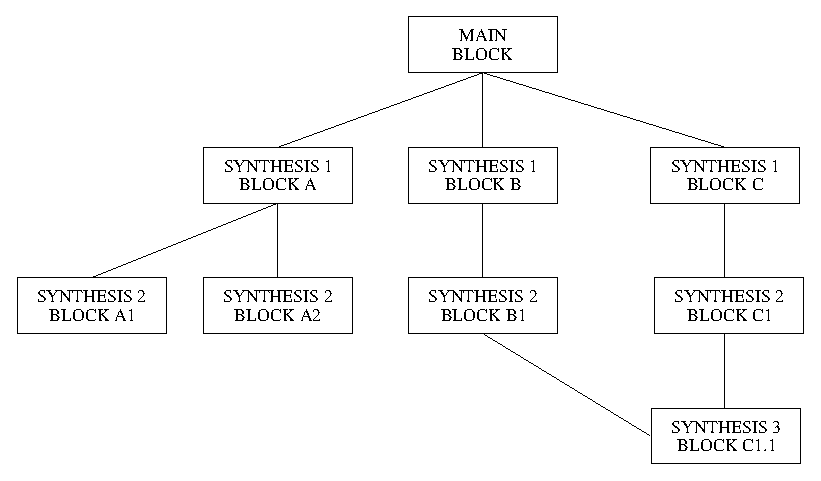
\includegraphics[scale=0.5]{figures/ed.eps}
	\caption{Object oriented design.}
	\label{fig:sd}
\end{figure}

From the previous definition it is important to note the following: the object oriented design (1) guides to an object oriented decomposition and (2) makes use of different notations to express different models of the logical design (class and object architecture) and the physical design (modules and process architecture) of a system.

Structured Design (SD) is concerned with the development of modules and the synthesis of these modules in a so called "module hierarchy" \cite{pagejones}. In order to design optimal module structure and interfaces two principles are crucial:
\begin{itemize}
    \item Cohesion which is "concerned with the grouping of functionally related processes into a particular module"\cite{hecht}, and
    \item Coupling relates to "the flow of information, or parameters, passed between modules. Optimal coupling reduces the interfaces of modules, and the resulting complexity of the software".\cite{hecht}
\end{itemize}    

Object oriented design uses classes and abstractions of objects for logic structured systems; structured design uses algorithmic abstractions. The {\it object model} is made up four basic elements that allows to define the base where the OOP lies upon, these are \cite{joyanes},\cite{booch}:

\begin{itemize}
\item Abstraction - Abstraction is simplifying complex reality by modeling classes appropriate to the problem, and working at the most appropriate level of inheritance for a given aspect of the problem.
\item Encapsulation - In an object-oriented programming language encapsulation is used to refer to one of two related but distinct notions, and sometimes to the combination \cite{scott},\cite{dale} thereof:
	\begin{itemize}
    \item A language mechanism for restricting access to some of the object's components.\cite{mitchell},\cite{pierce}
    \item A language construct that facilitates the bundling of data with the methods operating on that data.\cite{connolly}
    \end{itemize}
\item Modularity - Concerns are separated such that no (or few) modules depend upon other modules of the system. To have as few dependencies as possible is the goal. When creating a modular system, instead of creating a monolithic application (where the smallest component is the whole application), several smaller modules are built (and usually compiled) separately that, when composed together, will construct the executable application program.
\item Hierarchy - Abstraction is useful but it is possible to find so many different abstractions, so many that it may be possible to understand them at the time. Encapsulation also helps providing a way to group abstractions logically related. Nevertheless, this is not enough. A group of abstractions makes a hierarchy, identifying those hierarchies greatly helps to understand the problem. Therefore, {\it hierarchy} is as ``an arrangement or ordering of abstractions''.
\end{itemize}

As for the structured design of electronic circuits the process consist, briefly, in dividing the problem into smaller problems which can be solved individually. Once these individual problems have been solved, all are being assembled back into the original entity and, as a result, providing an effective solution to the particular problem. The following sections will show that the electronic structured design methodology complies with the OOP. Thus, it will be possible to algorithmize and implement the methodology into a software tool

\section{Modified Nodal Analysis}


\section{Electronic Structured Design}
Electronic circuit design consists on the search through many component combinations each one with different kind of properties. It would be a burden of time to find the best circuit that solves {\it completely} the design requirements established through the seek and test methodology. An strategy to find the best solution in the shortest of time is a necessity. The {\it standard} strategy is to re-use an already working circuit and, by some changes in its parameters, is possible to solve the problem with new specifications \cite{verhoeven}. The way the circuit behaves under certain circumstances will determine if this new design is implemented or discarded. If the design is discarded, the process is started over once again.

Even though the ``normal'' strategy sooner than later will provide useful results, there are several disadvantages in it:

\begin{itemize}
\item This strategy never guarantees that the solution found is the {\it optimum} solution to the problem and does not provide information on how close it may be.
\item The relationship between component parameters and circuit performance is not entirely explicit. In an incidental way, the circuit performance could be sensitive to an irrelevant parameter due to the fact that the employed circuit is not adequate for the selected task.
\item It is too complicated to determine what should be modified in the circuit when, for instance, specifications are modified.
\end{itemize}

To create order from the caos that the amplifier design is, the design is divided into smaller, orthogonal problems as possible. This way it is possible to clarify what the problem is and ease the way on how will be solved. The {\it electronic structured design} methodology \cite{verhoeven}, \cite{nordholt} allows to find {\bf ONE} solution to the design problem in a fast way (Figure \ref{fig:sd_1}). Nevertheless, this method is based on a certain amount of supositions and a limited quantity of rules. Therefore, the application of the electronic structured design should never support the dogmatic rejection of the results obtained by designs created using the ``normal'' (or results obtained by means of some other strategy) since it would be a stepback on the evolution of the design theory.

\begin{figure}[hbtp]
	\centering
	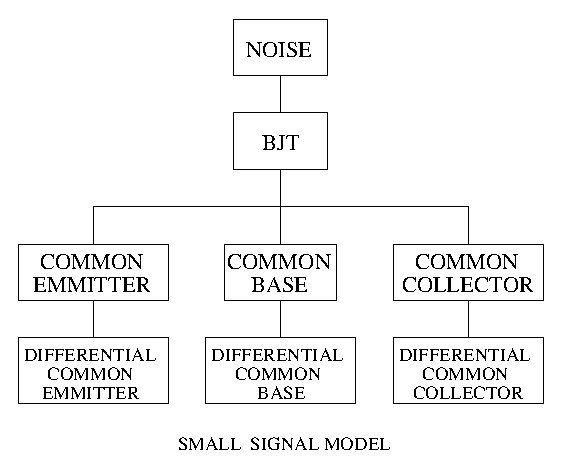
\includegraphics[scale=.65]{figures/bloque_ruido.eps}
	\caption{Example of Circuit Structured Design.}
	\label{fig:sd_1}
\end{figure}

The amplifier structured design methodology focus on three fundamental aspects to perform the behavioral circuit description

\begin{itemize}
\item Noise.
\item Distortion.
\item Bandwidth.
\end{itemize}

In order to speed-up the design process,some suppositions should be done, as said before. These will be assessed according to the basic specifications that should be provided, on the circuit behavior based on the results using simple models, and to the decisions taken on each design stage in particular. This design methodology is based on three basic elements: 

\begin{itemize}
\item Orthogonality - Circuits will be ordered in such a way that behavior of the three fundamental aspects can be designed in an orthogonal fashion, that is, el behavior of one stage will not have any influence on the other two.
\item Simplicity - Simple models are defined to obtain fast predictions of the feasibility of the design. Non-viable solutions will be detected on early stages of the design. Special planning should be done to allow the ``estimated'' results be the ``closest'' as possible to the real values.
\item Hierarchy - Hierarchy allows design to decrease the design problem complexity because allows its efficient division into smaller and independent design problems. Planning on this matter should be done in a way that decision taken in certain hierarchical level should keep valid for the rest of design.
\end{itemize}

\section{Relating OOP with ESD}
Because the electronic design technique contains the phrase ``structured'' does not imply that it fulfills the basic principles of the object oriented design; this section will show that it not only complies with the fundamentals of the OOD but it can also be broaden to the OOP and, in the end, create on automated design software tool.

The electronic structured design (ESD) complies with the principle of the object oriented design (OOD) since it is a process that decompose a problem (block) in a certain number of smaller problems (blocks), which can also be sub-divided and this process can continue until the specific problem is isolated. Once the relationship with the OOD has been stablished, it is now time to upgrade this idea up to the OOP concept. A good starting point is that both techniques employ the hierarchy idea on the design process, this will simplify the feasibility to propose hierarchical models that can be converted in useful model for the OOP. The complexity of the models should no be modified, that is, in a first approach simple model are employed in prelimiary tests and on succesful results the complexity of the models will be upgraded and substituted.


For the abstraction concept the structured design does not have a similar concept. Nevertheless, does have an element that can be employed as some kind of abstraction. The nullor, ideal element from which the design problem solution starts, may be considered an abstraction element. This element could be taken as {\bf entity abstraction} \cite{booch}, and refers that an object represents a useful model within the domain of the problem. As for the OOP, its focus on this matter is to use entity abstraction also.

Modularity of the OOP has its counterpart on the structured design on the {\bf orthogonality}. The design is dividen in three parts to achieve the nullor synthesis (noise, bandwidth, and distortion). Once the division has taken place, it is possible to subdivide each one of these parts. When all the small problems have been solved, the reverse process is carried out and these parts are ``glued'' together once again until the main block is restored (the synthesized nullor). This fullfills the modularity definition in OOP. (Figure \ref{fig:nullor_1}). 

\begin{figure}[hbtp]
	\centering
	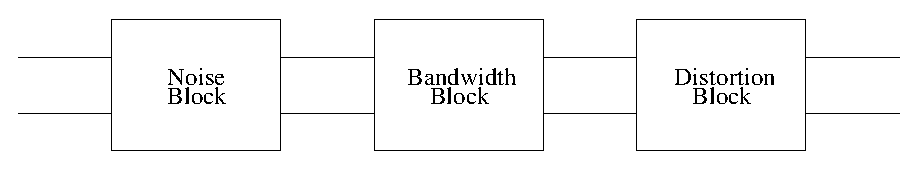
\includegraphics[scale=0.5]{figures/basic_blocks.eps}
	\caption{Dividing the modules to be synthesized.}
	\label{fig:nullor_1}
\end{figure}

The encapsulation for the structured design is a concept not so simple to implement on the strict sense of the concept. One alternative could be, once again, to use the nullor and its different syntehsis stages. Given the fact that the nullor is an ideal element, it is necessary the implement it using ``real'' devices. The synthesis of the first stage (noise) on the highest hierarchy it can be seen the nullor within the amplification circuit. Adding the second synthesized stage (distortion) it can be seen as just one block. Within this nullor there are several active devices (BJT's, MOSFET's) but in a lower hierarchy. This way it is possible to ``hide'' all the details of the objects that take part on the implementation. (Figure \ref{fig:nullor}).

\begin{figure}[hbtp]
	\centering
	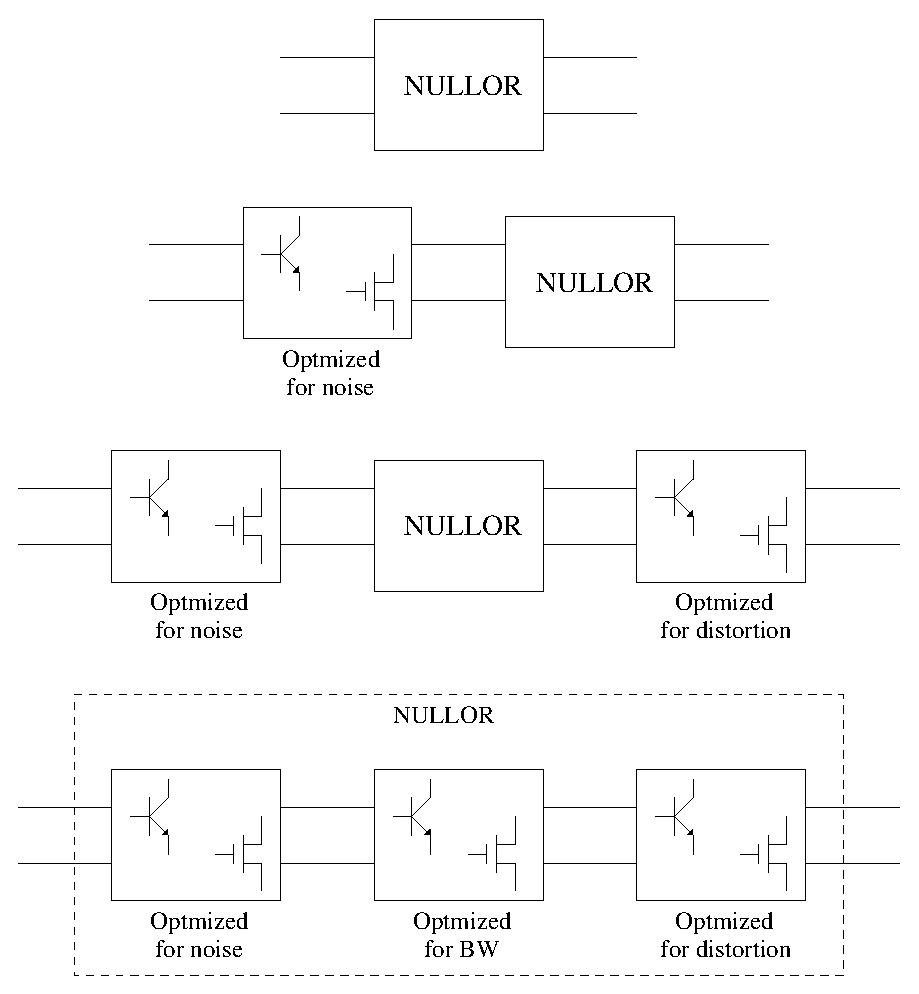
\includegraphics[scale=.5]{figures/synthesis_process.eps}
	\caption{Encapsulation applied to the nullor synthesis.}
	\label{fig:nullor}
\end{figure}

\section{CAD Tool Structure}
Given the basic blocks that structured design is based on to create an amplifier, a rather general structure for the design based on these blocks is shown in Figure \ref{fig:descad}. This tool has been developed under the code name {\it Descad\_Wizard} to reflect that the adequate way to operate this tool is using a {\it wizard} approach, that is, development process is performed by filling up some options within a window. Calculations are programmed in C++ \cite{joyanes} and the graphical user interface is provided by Qt \cite{qt}. 

\begin{figure}[hbtp]
	\centering
	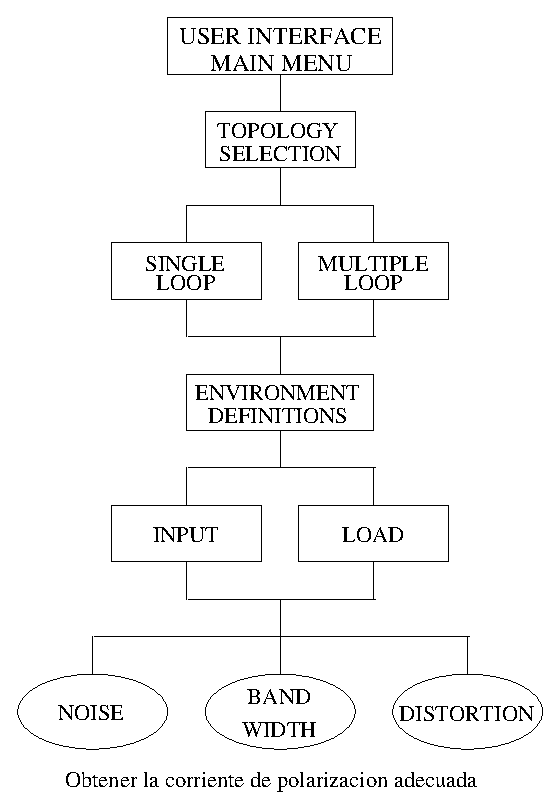
\includegraphics[scale=0.5]{figures/descad_1.eps}
	\caption{General structure for the CAD tool.}
	\label{fig:descad}
\end{figure}

Figure \ref{fig:des1} shows the first window where basic specifications are typed. Basic requirements refers to the basic amplifier structure like:

\begin{itemize}
\item Amplifier types.
\item Amplifier configuration.
\item Source and load types and values.
\item Gain and sign specs.
\end{itemize}

\begin{figure}[hbtp]
	\centering
	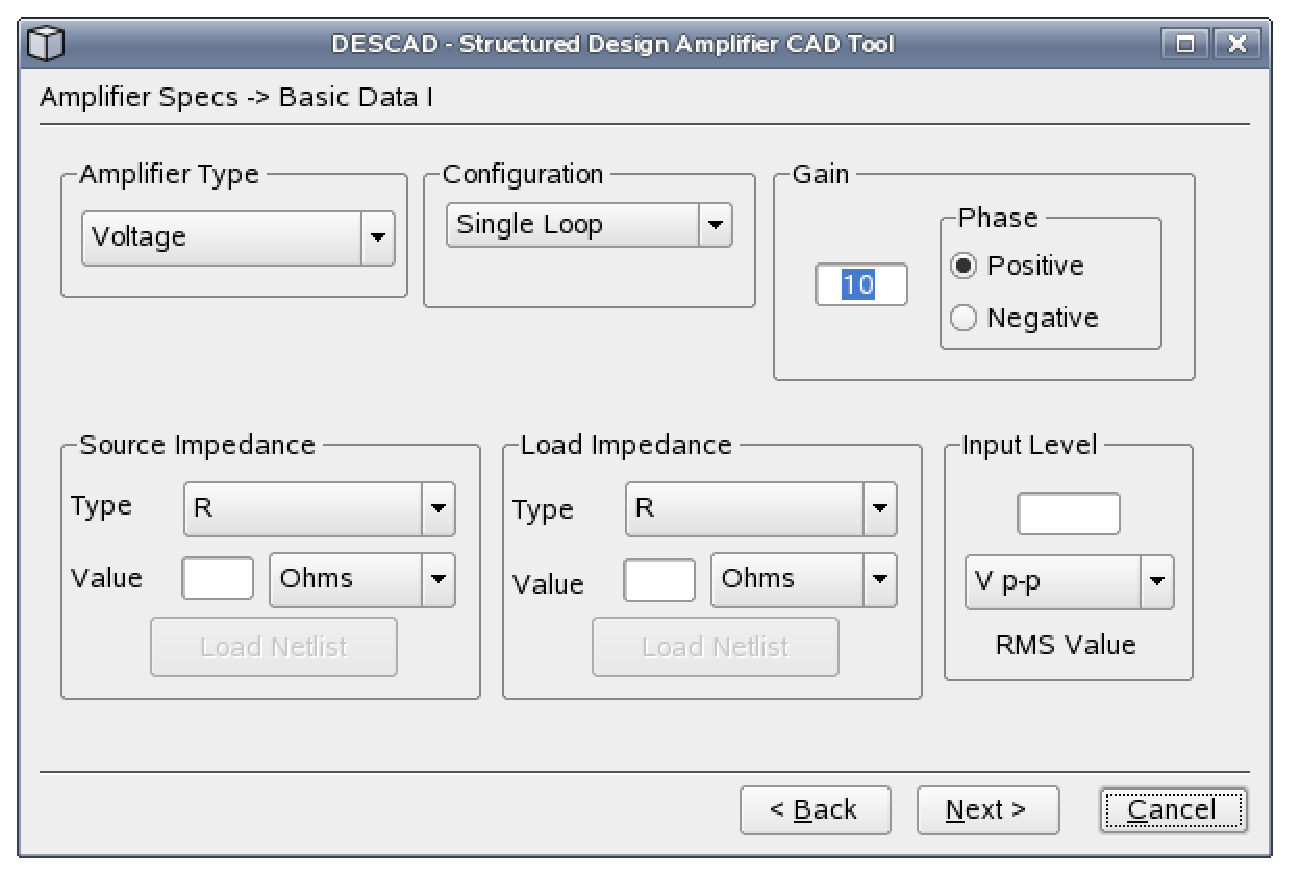
\includegraphics[scale=0.3]{figures/step1.eps}
	\caption{Basic specifications window.}
	\label{fig:des1}
\end{figure}

The gain value can be provided as a floating-point number or in scientific format; phase value refers to the output phase that is desired at the output port of the amplifier. Phase can be positive (no phase change) or negative (phase is shifted $180\,^{\circ}$ away). Another specification to be provided is the desired configuration, it could be one of two options. First option is to select one of the single-loop amplifiers: (1) voltage amplifier, (2) transconductance amplifier, (3) transresistance amplifier and (4) current amplifier. These amplifiers are depicted in Figure \ref{fig:amps}. Second option is a two-loop amplifier. This type of amplifier comprises the transconductance and transresistance amplifiers. Figure \ref{fig:two_loop}.

\begin{figure}[hbtp]
	\centering
	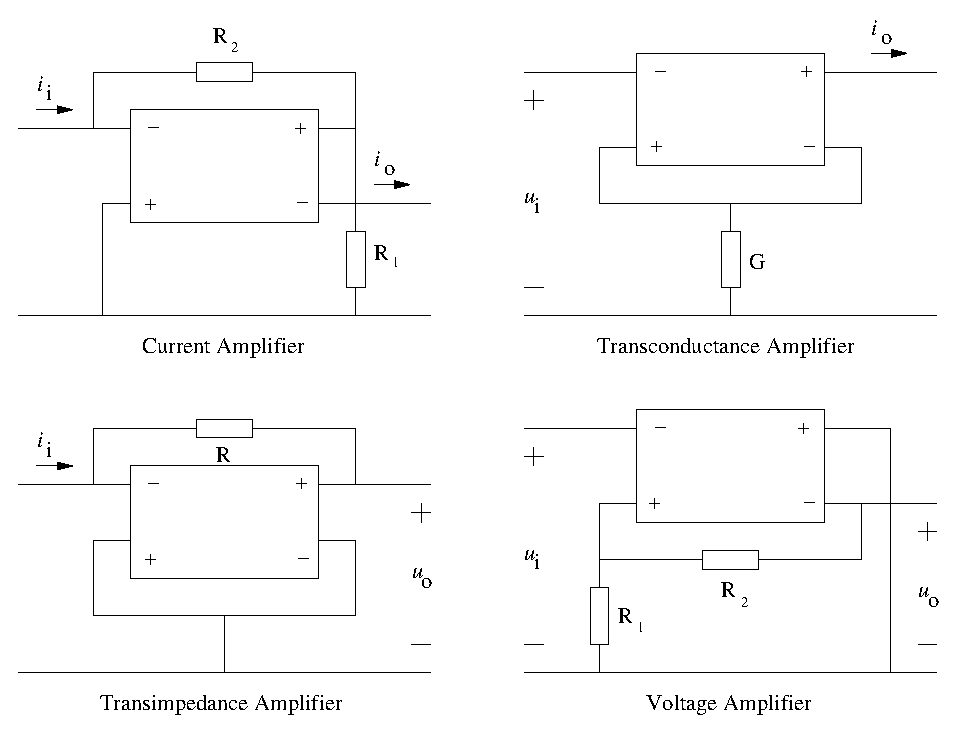
\includegraphics[scale=0.5]{figures/grupo_eng.eps}
	\caption{Amplifier types.}
	\label{fig:amps}
\end{figure}

\begin{figure}[hbtp]
	\centering
	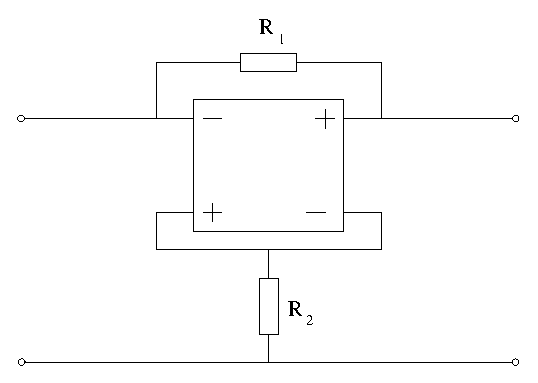
\includegraphics[scale=0.5]{figures/twoloop_basica.eps}
	\caption{Two-loop amplifier topology.}
	\label{fig:two_loop}
\end{figure}

For the synthesis of noise, clipping and bandwidth stages a scheme is provided in Figure \ref{fig:descad2}. It means that for every stage it is possible to choose a single device or differential (two devices) configurations; it is worth noting that in order to keep the negative feedback behaviour a differential configuration must be placed either on noise or clipping stages. Windows for the noise and clipping stages are depicted in Figure \ref{fig:descad3} and Figure \ref{fig:descad4}.

\begin{figure}[hbtp]
	\centering
	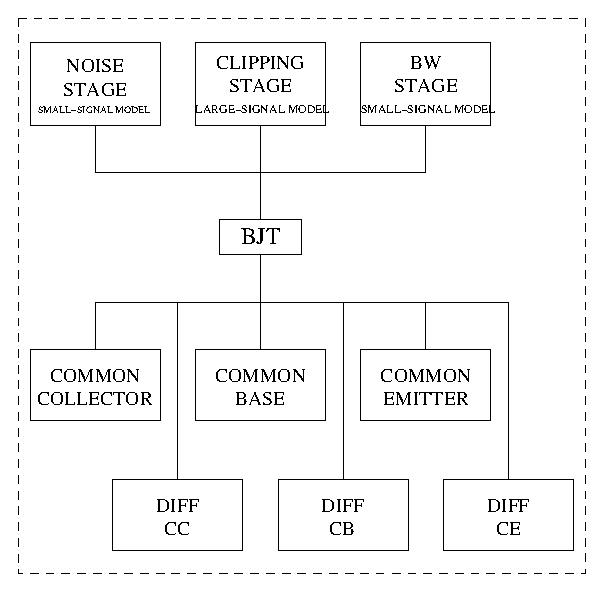
\includegraphics[scale=0.5]{figures/descad2.eps}
	\caption{Noise, clipping and bandwidth synthesis scheme.}
	\label{fig:descad2}
\end{figure}

\begin{figure}[hbtp]
	\centering
	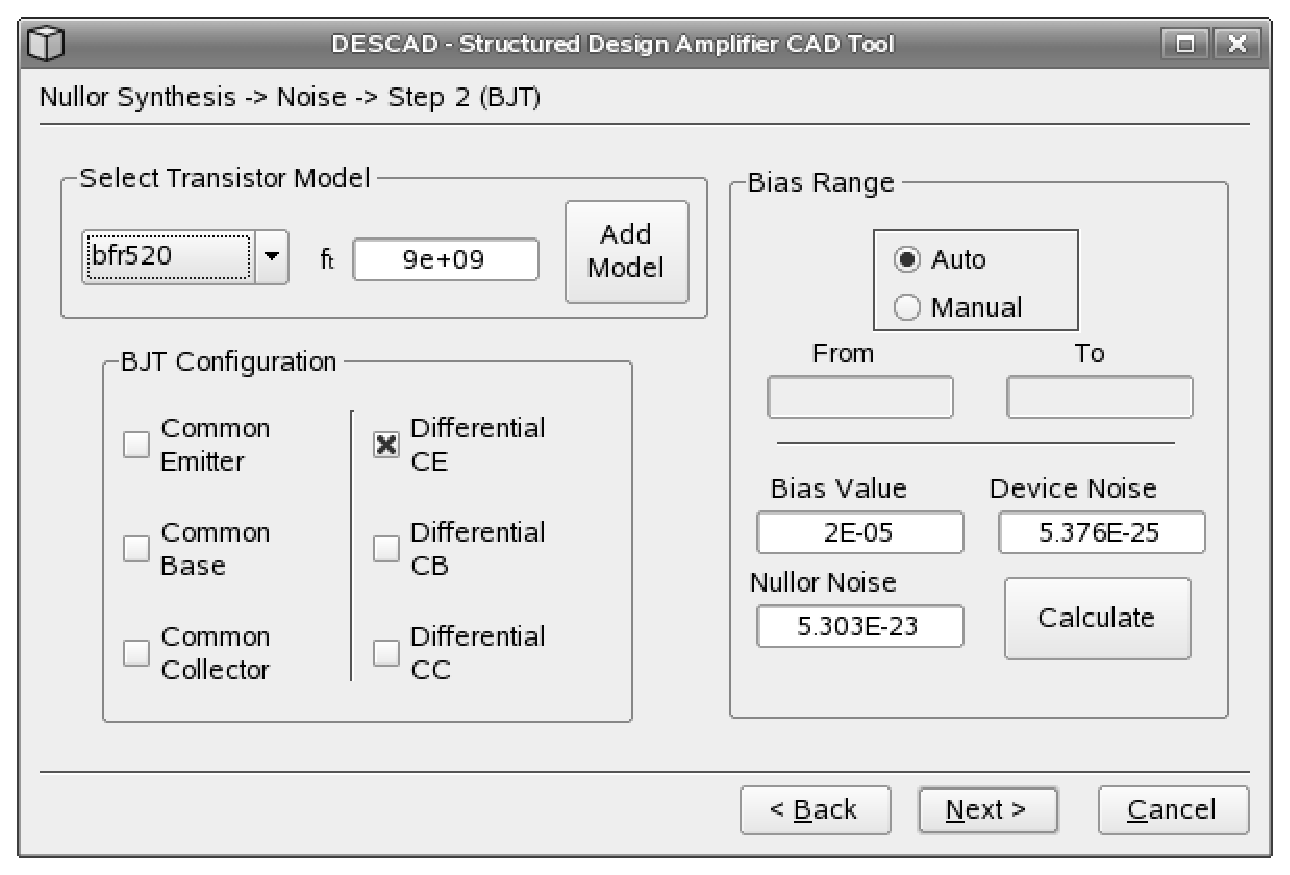
\includegraphics[scale=0.3]{figures/wizard3.eps}
	\caption{Noise stage window.}
	\label{fig:descad3}
\end{figure}

\begin{figure}[hbtp]
	\centering
	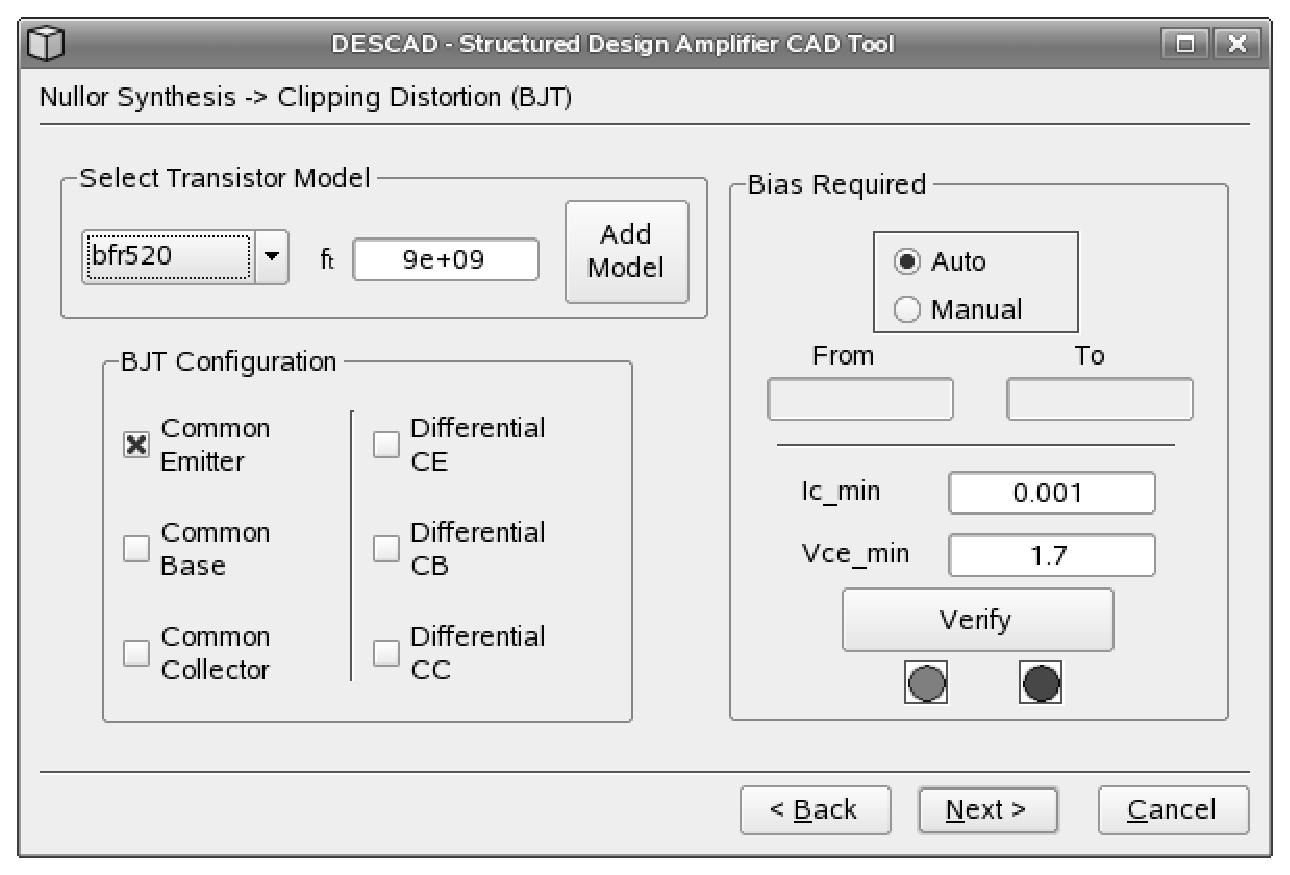
\includegraphics[scale=0.3]{figures/wizard4.eps}
	\caption{Clipping stage window.}
	\label{fig:descad4}
\end{figure}

Bandwidth synthesis process is divided in two steps: (1) calculate the LP-product \cite{verhoeven} in order to verify if design is capable to handle the desire bandwidth and (2) in order to guarantee a flat output frequency response, amplifier poles must be located at Butterworth locations \cite{nordholt}. In case that the LP-product is not high enough for the desired bandwidth, there are three options to be applied in this order: (1) increase collector current for the noise stage as high as the noise behaviour is kept within constraints. (2) If the LP-product is still low, an increase on the collector current for the clipping stage is performed. This increase can only be applied if clipping is below the allowed value. (3) Last case is to add another device to the design increasing the amplifier degree by 1. Figure \ref{fig:descad5} shows the LP-product window.

\begin{figure}[hbtp]
	\centering
	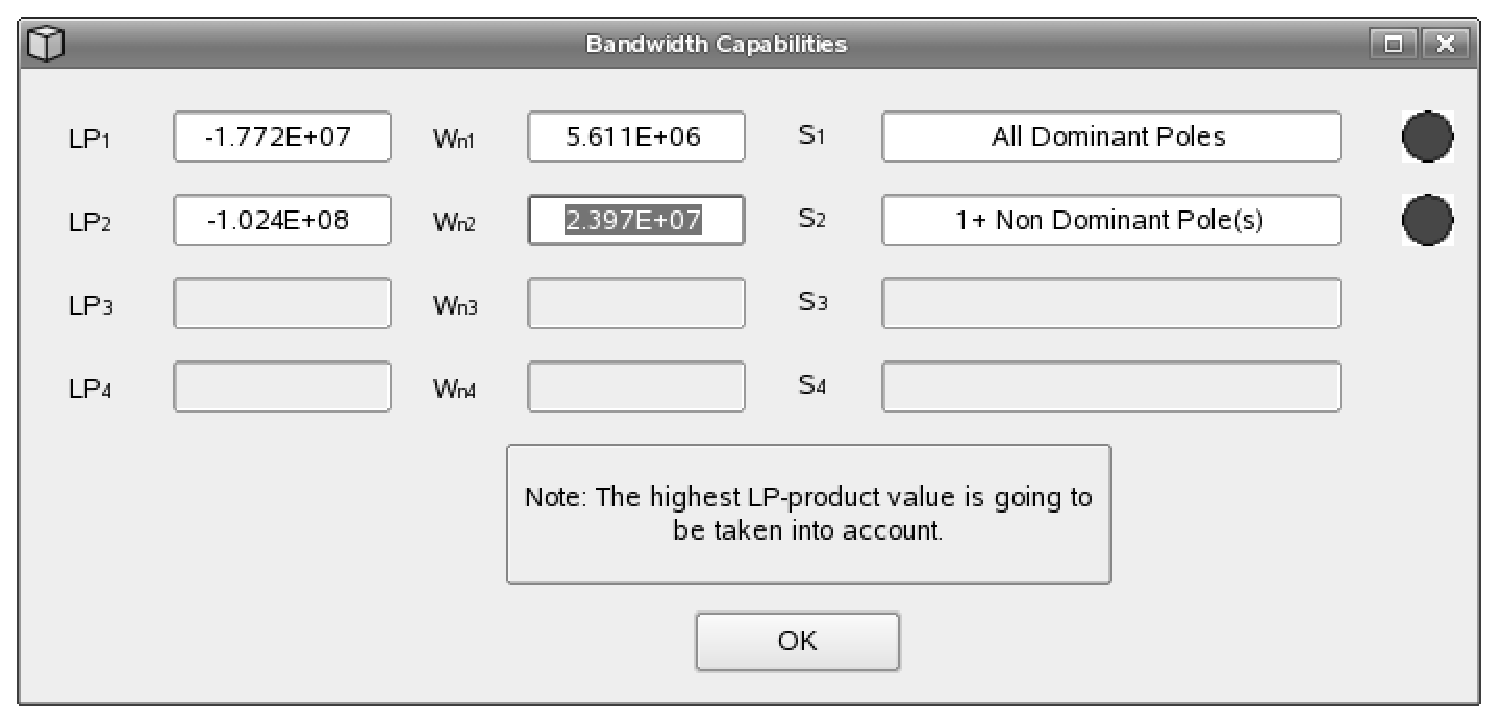
\includegraphics[scale=0.3]{figures/wizard5.eps}
	\caption{The LP-product window.}
	\label{fig:descad5}
\end{figure}

Once the LP-product is high enough the process to place the closed-loop poles of the amplifier in Butterworth position is performed. \cite{verhoeven} and \cite{nordholt} provide the adequate compensation techniques in order to place the amplifier poles at the required location. Given the fact that it is possible to perform compensation at the input port, output port and feedback network the user is capable to select where to perform the compensation. Nevertheless if compensation fails to adjust the poles position, a warning message is displayed and the option is disabled then the user must select any available option. Figure \ref{fig:descad6}.

\begin{figure}[hbtp]
	\centering
	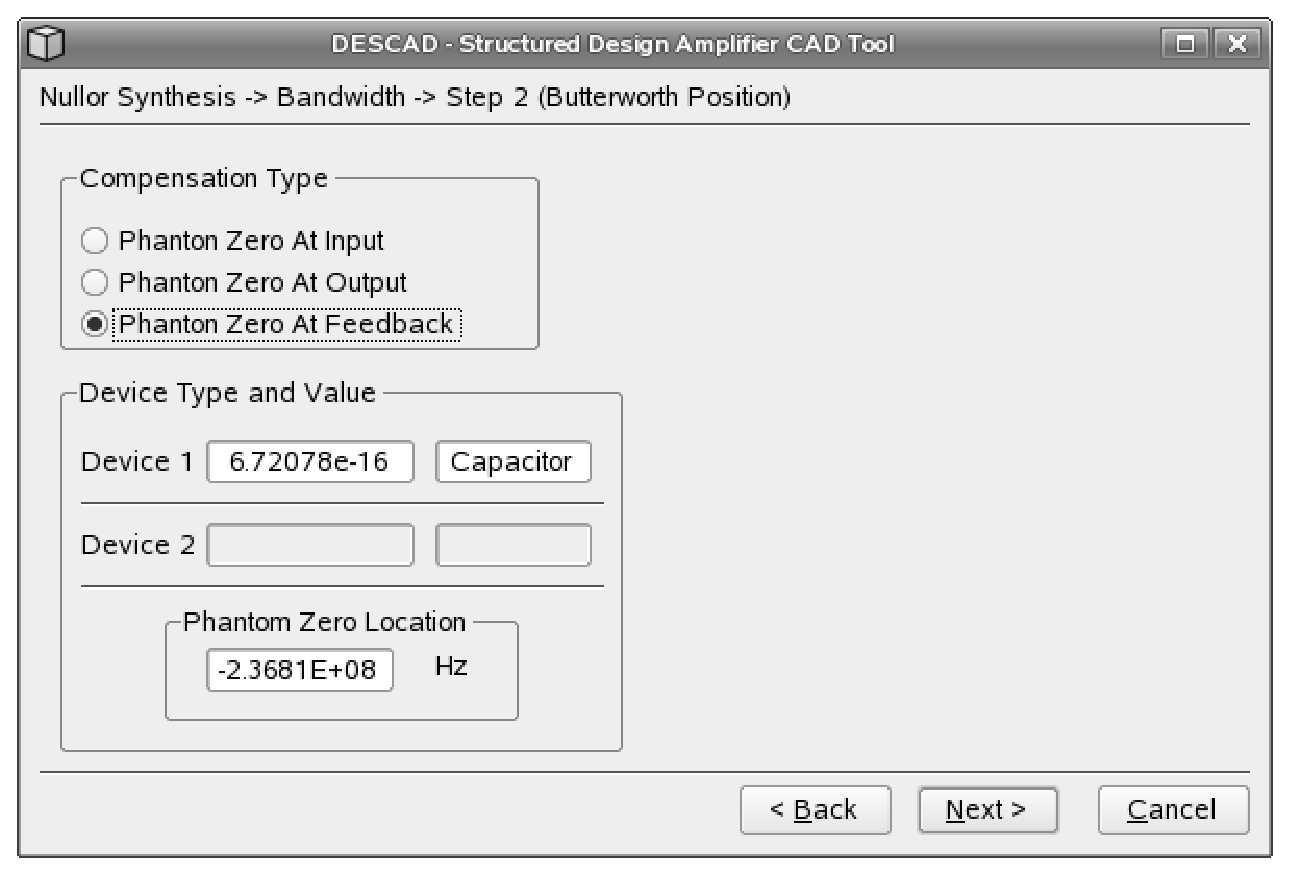
\includegraphics[scale=0.3]{figures/wizard6.eps}
	\caption{Butterworth compensation stage.}
	\label{fig:descad6}
\end{figure}

Finally a summary is displayed providing the constraints given by the user and the results of the synthesis procedure. Besides an input file for an industrial simulator is generated. Figure \ref{fig:descad7}.

\begin{figure}[hbtp]
	\centering
	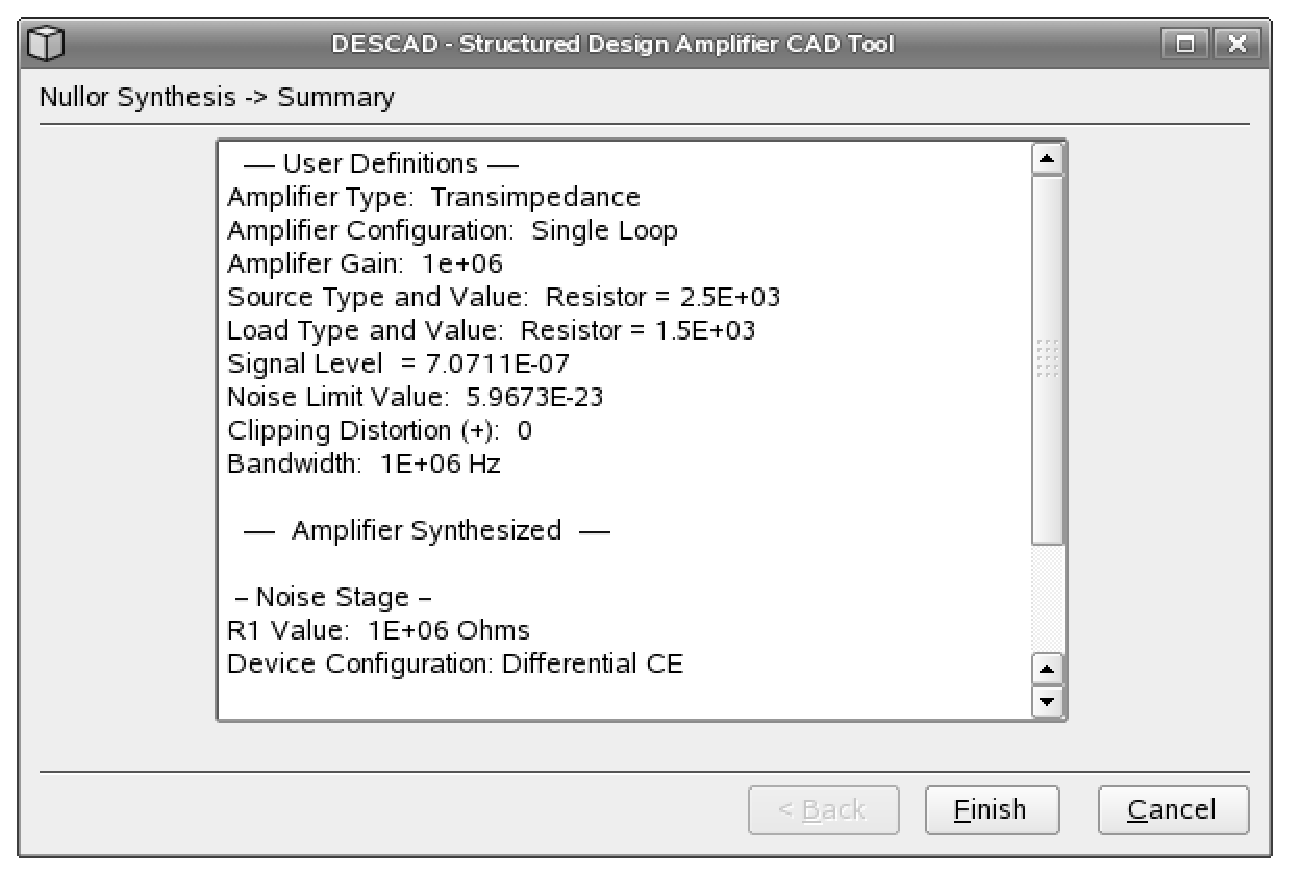
\includegraphics[scale=0.3]{figures/wizard8.eps}
	\caption{Design summary window.}
	\label{fig:descad7}
\end{figure}

\section{Example}
As an example a transconductance amplifier is going to be designed and must satisfy these constraints:

\begin{itemize}
\item Source Type and Value: Resistor - $5K{\Omega}$
\item Load Type and Value: Resistor - $1.5K{\Omega}$
\item Input Level: .5 $\mu$A
\item Output Level: .5 V
\item Noise Level: 10 dB
\item Clipping: 0 \%
\item Bandwidth: 1 MHz
\end{itemize}

Noise values calculated for the feedback and source impedances:

\begin{itemize}
\item Source Noise: 3.315E-24 $A^2/Hz$
\item Feedback Noise: 1.658E-26 $A^2/Hz$
\end{itemize}

The nullor synthesis for the noise stage is performed with the transistor BFR520 \cite{bfr520} in differential common emitter configuration. The minimum $I_C$ and noise values are: 

\begin{itemize}
\item $I_C=2E-5\;A$
\item Noise=1.351E-25 $A^2/Hz$
\end{itemize}

Clipping distortion stage synthesis is provided by the transistor BFR520 in common emitter configuration. Values are:

\begin{itemize}
\item $I_C=0.001\;A$
\item $V_{CE}=1.7$ V
\end{itemize}

Note that values on the clipping stage are compared to the maximum allowable values taken from the device datasheet. For the bandwidth stage and the LP-product calculation process on the first run the result was that the LP-product is high enough but had one or more non dominant poles. This behaviour is not desired because affects the overall gain, consequently an adjustment is required. The adjustment is performed on the noise stage because it has the best $I_C$ range. Consequently the new values for the noise stage are:

\begin{itemize}
\item $I_C=0.001\;A$
\item Noise=3.226E-26 $A^2/Hz$
\end{itemize}

Hence for the Butterworth compensation process it is performed at the feedback network. In this case a capacitor is placed in parallel to the feedback resistor and its value is $C=9.50872E-16$F.

Simulation on the amplifier circuit is performed using HSpice \cite{hspice}. Instead of using the actual active device, \mbox{small-signal} elements are employed. Small-signal values are calculated using the $I_C$ found for each synthesised stage. Figure \ref{fig:sim} shows the resulting. As it can be seen a flat output behaviour is achieved on the desired frequency.

\begin{figure}[hbtp]
	\centering
	\includegraphics[scale=0.3,angle=-90]{figures/iced_2006.ps}
	\caption{Amplifier simulation output.}
	\label{fig:sim}
\end{figure}

\bibliography{bib/jsea_journal}
\bibliographystyle{ieeebib}
\end{document}